\documentclass[../main.tex]{subfiles}
\begin{document}
\begin{figure}[H]
	\begin{tabular}{ccc}
		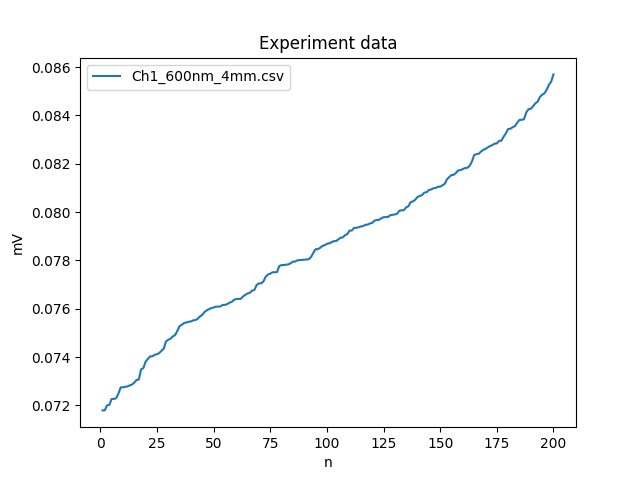
\includegraphics[scale=0.5]{figures/input_PR1.png}
		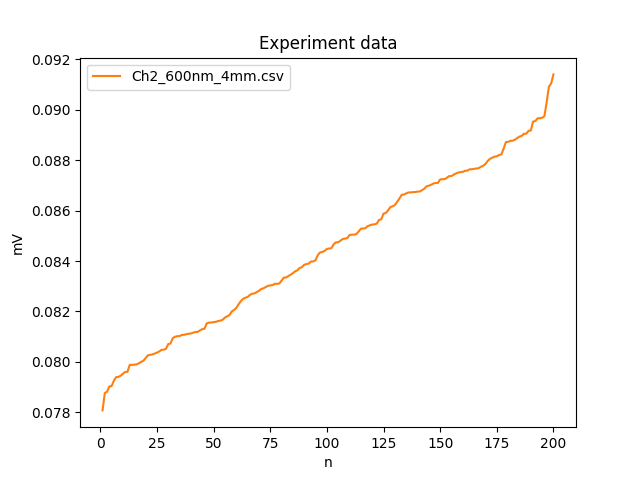
\includegraphics[scale=0.5]{figures/input_PR2.png}
	\end{tabular}
	\caption{Исходные данные из экспериментов} 
\end{figure}

\begin{figure}[H]
	\begin{tabular}{ccc}
		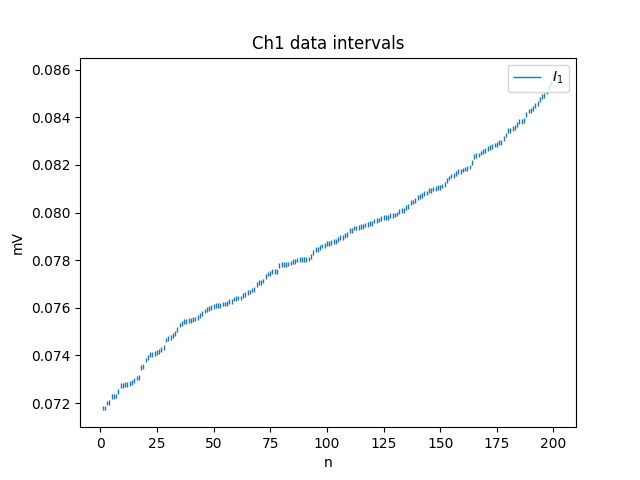
\includegraphics[scale=0.5]{figures/intervals_PR1.png}
		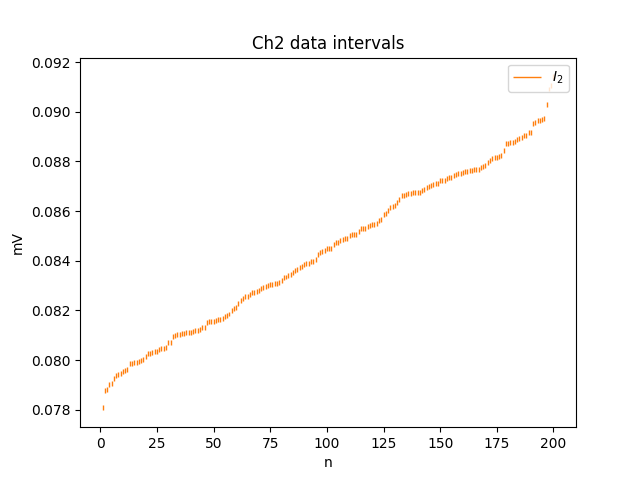
\includegraphics[scale=0.5]{figures/intervals_PR2.png}
	\end{tabular}
	\caption{Интервальное представление исходных данных} 
\end{figure}

\begin{figure}[H]
	\begin{tabular}{ccc}
		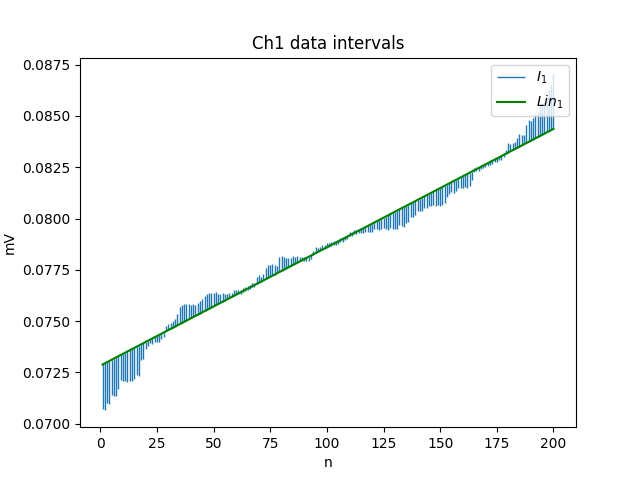
\includegraphics[scale=0.5]{figures/lr_PR1.png}
		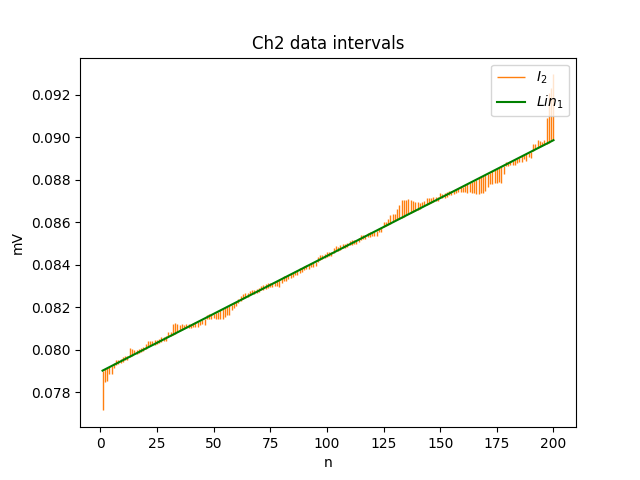
\includegraphics[scale=0.5]{figures/lr_PR2.png}
	\end{tabular}
	\caption{Линейная модель дрейфа данных} 
\end{figure}

\begin{figure}[H]
	\begin{tabular}{ccc}
		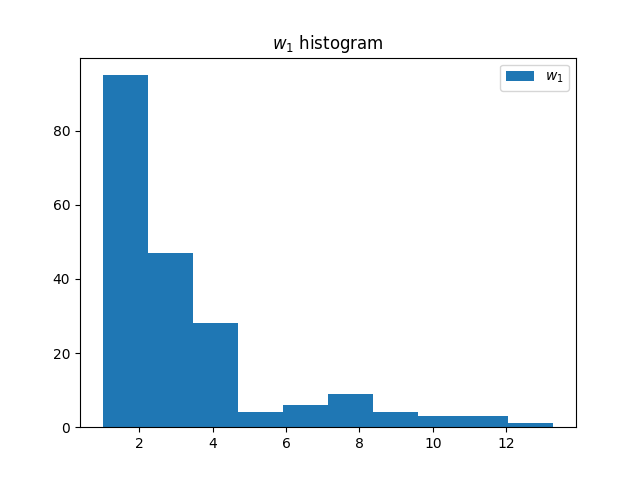
\includegraphics[scale=0.5]{figures/whyst_PR1.png}
		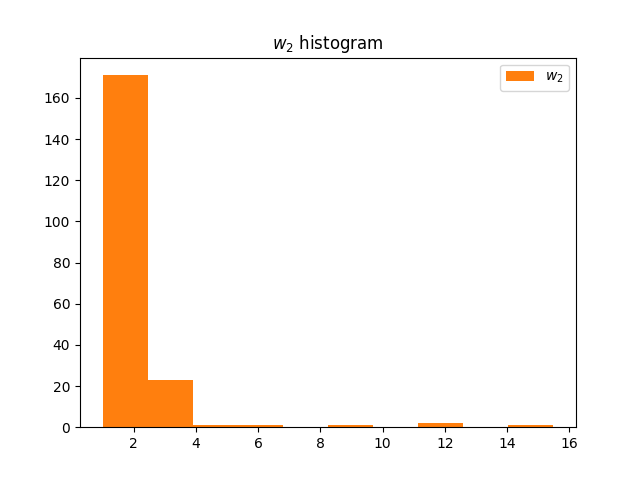
\includegraphics[scale=0.5]{figures/whyst_PR2.png}
	\end{tabular}
	\caption{Гистограммы значений множителей коррекции w} 
\end{figure}

Результаты линейного приближения токов:
\begin{itemize}
\item Первый фотоприемник
        \begin{equation}
            A_1 = 0.0728307
        \end{equation}
        
        \begin{equation}
            B_1 = 5.76887e-05
        \end{equation}

\item Второй фотоприемник
        \begin{equation}
            A_2 = 0.0789563
        \end{equation}
        
        \begin{equation}
            B_2 = 5.44961e-05
        \end{equation}
\end{itemize}

\begin{figure}[H]
	\begin{tabular}{ccc}
		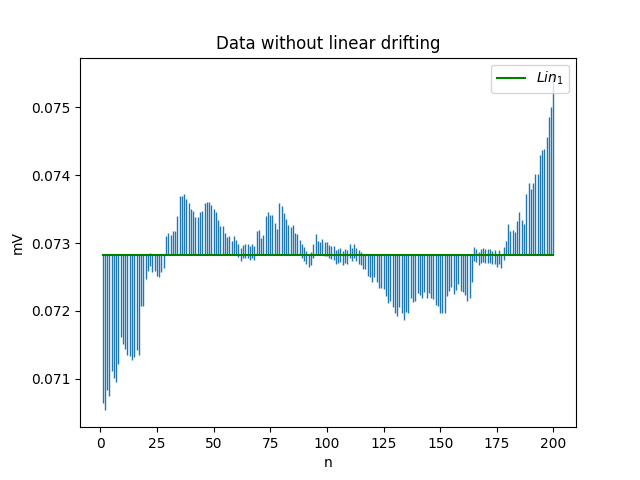
\includegraphics[scale=0.5]{figures/fixed_PR1.png}
		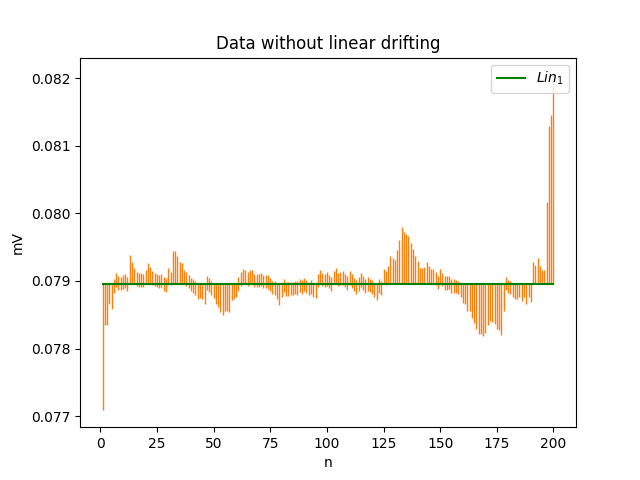
\includegraphics[scale=0.5]{figures/fixed_PR2.png}
	\end{tabular}
	\caption{Скорректированные модели данных} 
\end{figure}

\begin{figure}[H]
	\begin{tabular}{ccc}
		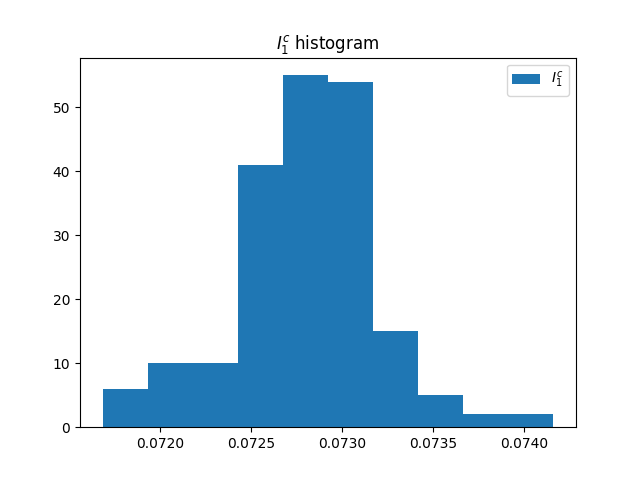
\includegraphics[scale=0.5]{figures/fhyst_PR1.png}
		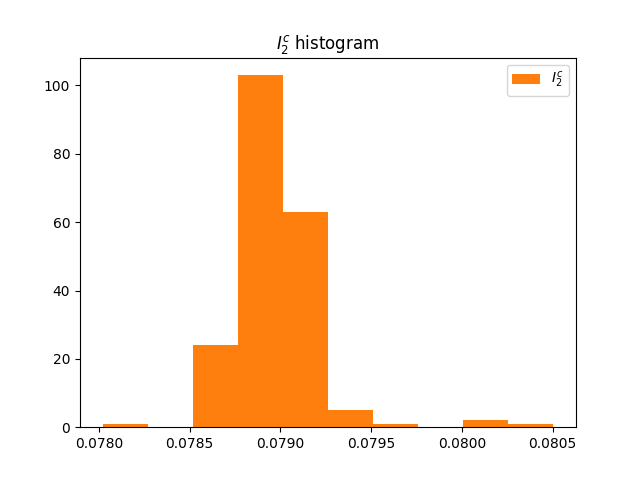
\includegraphics[scale=0.5]{figures/fhyst_PR2.png}
	\end{tabular}
	\caption{Гистограммы скорректированных данных} 
\end{figure}

\begin{figure}[H]
	\begin{center}{}
		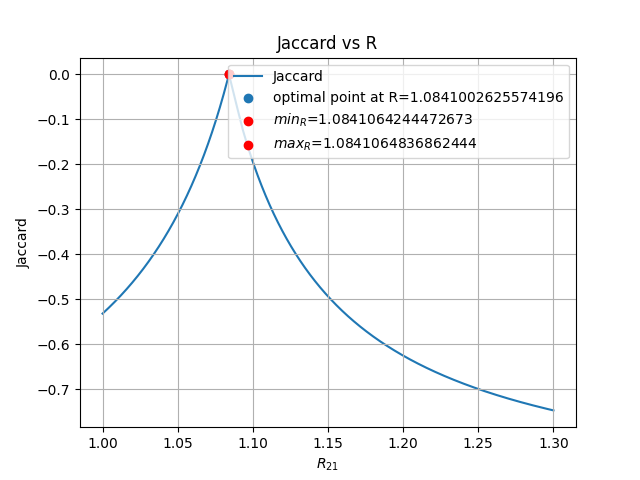
\includegraphics[scale=0.5]{figures/jakkar.png}
	\end{center}
	\caption{Значение коэффициента Жаккара от калибровочного множителя от $R_{21}$} 
\end{figure}
        \begin{equation}
            JK(x) = -0.11943227
        \end{equation}
        
        \begin{equation}
            R_{opt} = 1.0841
        \end{equation}


\begin{figure}[H]
	\begin{center}
		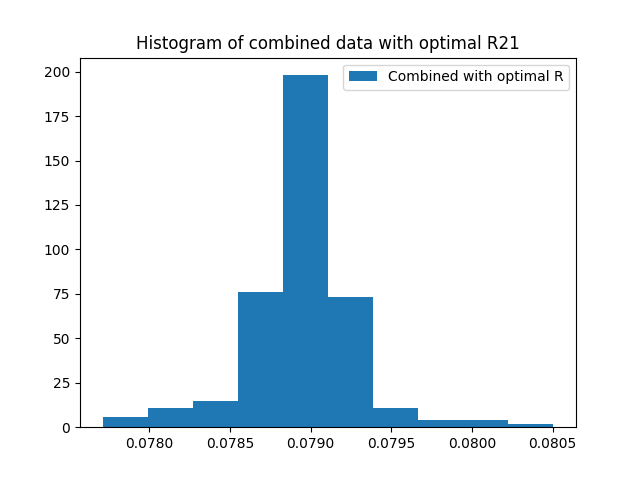
\includegraphics[scale=0.5]{figures/jakkar_combined_hist.png}
	\end{center}
	\caption{Гистограмма объединнённых данных при оптимальном значении $R_{21}$} 
\end{figure}
\end{document}